
The files *.slb contain slab contours of individual coherent slab bodies.
The first line contains a name which is the name of the file as they are
named here.  Subsequently come individual contours.  First the number of
samples on the contour.  Then longitude (0-360), latitude, and depth.
The contours are drawn such that they follow approximately the top of
the seismogenic region.


\begin{center}
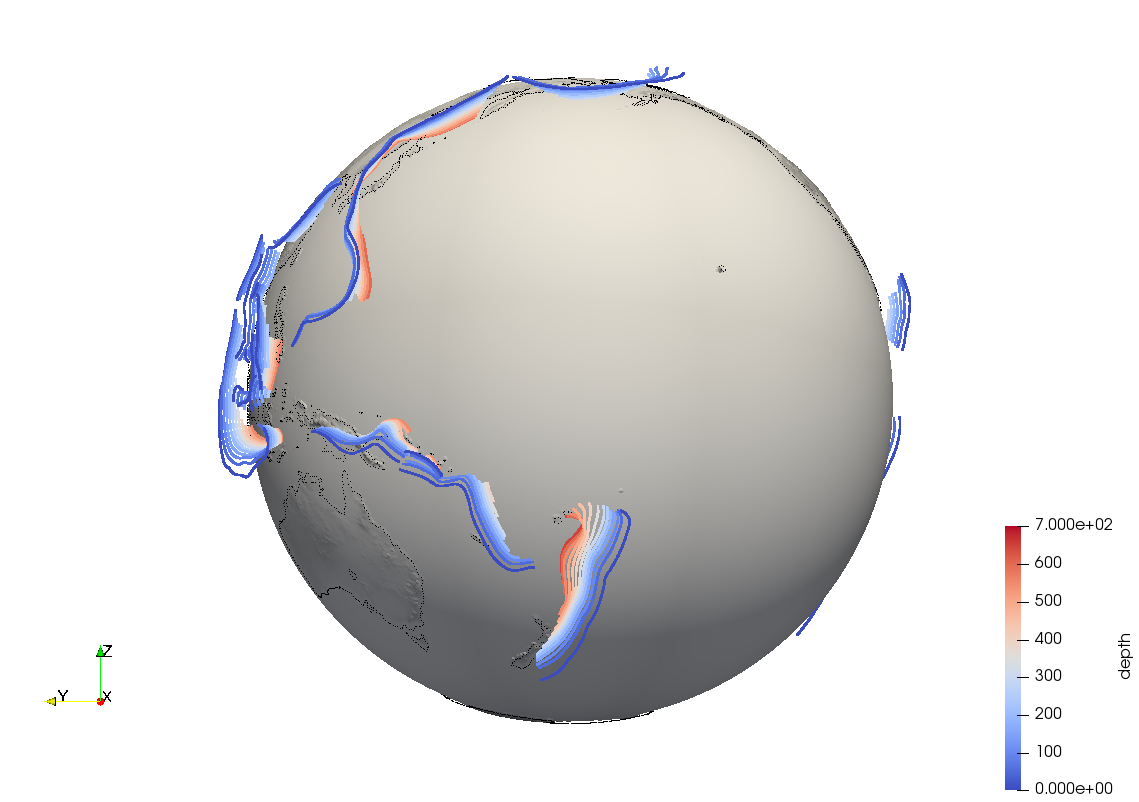
\includegraphics[width=7cm]{python_codes/fieldstone_136/view1}
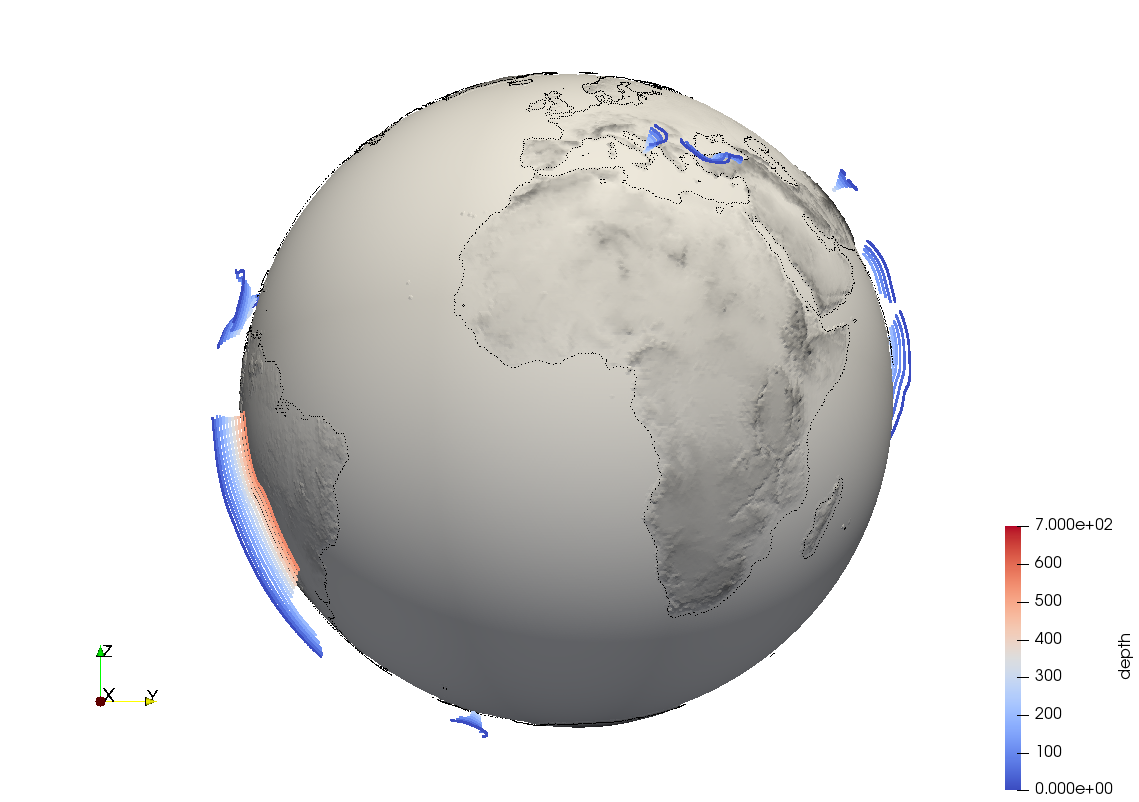
\includegraphics[width=7cm]{python_codes/fieldstone_136/view2}\\
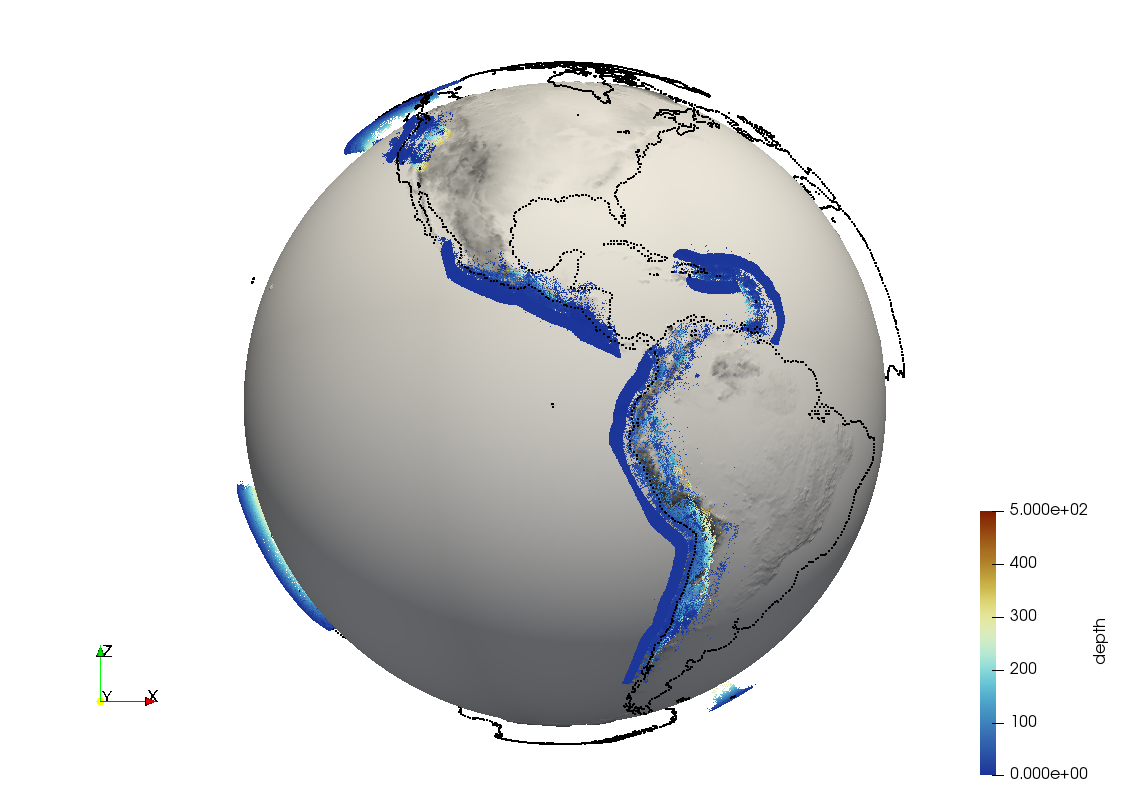
\includegraphics[width=7cm]{python_codes/fieldstone_136/view3}
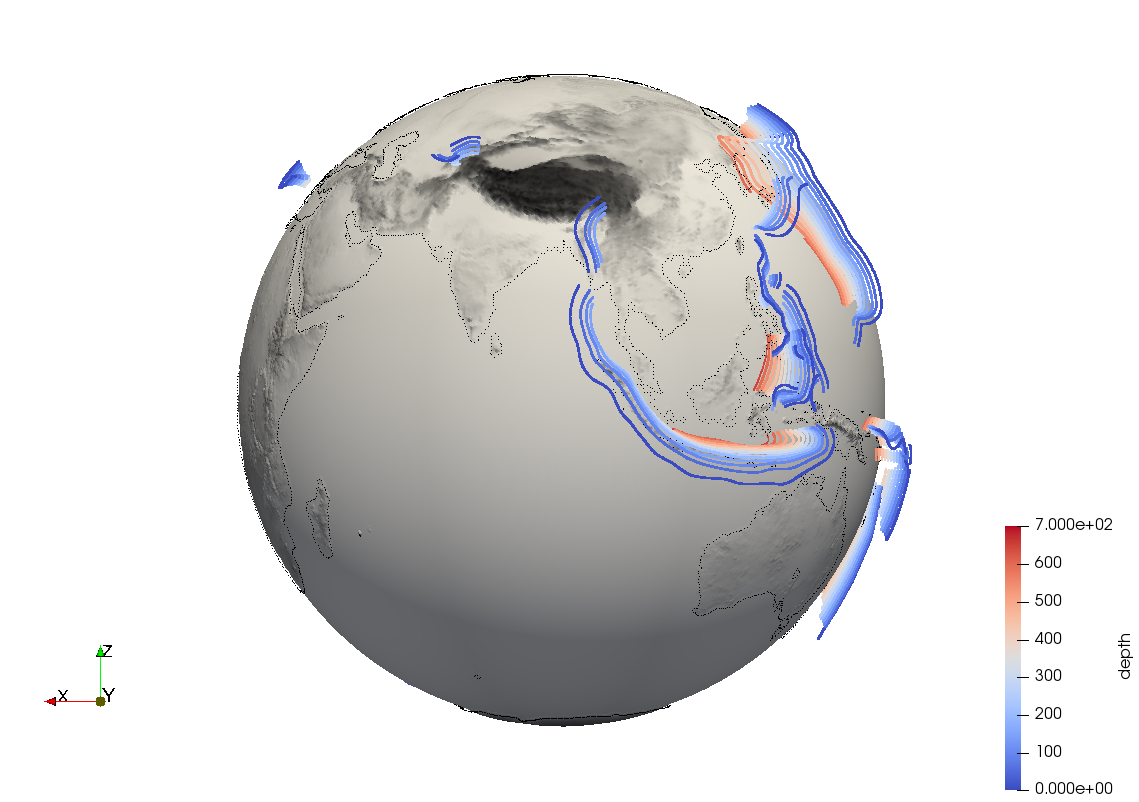
\includegraphics[width=7cm]{python_codes/fieldstone_136/view4}
\end{center}
